%%%%%%%%%%%%%%%%%%%%%%%%%%%%%%%%%%%%%%%%%%%%%%%%%%%%%%%%%%%%%%%%%%%%%%%%%
\section{Well-Posed Inference} %%%%%%%%%%%%%%%%%%%%%%%%%%%%%%%%%%%%%%%%%%
\label{cr:sec:inference}
% https://en.wikipedia.org/wiki/Well-posed_problem

The shortcomings of the MLE discussed in the previous section drive us to seek a more robust estimator.
Following the ideas of \citet{caron2012efficient}, we introduce an independent Gamma prior on each parameter, i.e., i.i.d. $\gamma_1, \ldots, \gamma_N \sim \DGamma{\alpha, \beta}$.
Adding the log-prior to the log-likelihood, we can write the log-posterior as
\begin{align}
\label{cr:eq:logpost}
\log p(\bm{\gamma} \mid \mathcal{D}) =
    \sum_{i = 1}^N \bigg[ (c^-_i + \alpha - 1) \log \gamma_i
        - c^+_i \log \bigg( \sum_{k \in \mathcal{N}^+_i} w_{ik} \gamma_k \bigg)  - \beta \gamma_i \bigg]
    + \kappa.
\end{align}
The Gamma prior translates into a form of regularization that makes the inference problem well-posed, as shown by the following theorem.

\begin{theorem}
\label{cr:thm:map}
If i.i.d. $\gamma_1, \ldots, \gamma_N \sim \DGamma{\alpha, \beta}$ with $\alpha > 1$, then the log-posterior~\eqref{cr:eq:logpost} always has a unique maximizer $\bm{\gamma}^\star \in \mathbf{R}^N_{>0}$.
\end{theorem}

\begin{proof}
Under the reparametrization $\gamma_i = e^{\theta_i}$, the log-prior and the log-likelihood become
\begin{align*}
\log p(\bm{\theta})
    &= \sum_{i = 1}^N \left[ (\alpha - 1) \theta_i - \beta e^{\theta_i} \right] + \kappa \\
\ell(\bm{\theta} ; \mathcal{D})
    &= \sum_{i = 1}^N \bigg[ c^-_i \theta_i - c^+_i \log \sum_{k \in \mathcal{N}^+_i} w_{ik} e^{\theta_k} \bigg] + \kappa.
\end{align*}
It is easy to see that the log-likelihood is concave and the log-prior strictly concave in $\bm{\theta}$ (for $\alpha > 1$).
As a result, the log-posterior is strictly concave in $\bm{\theta}$, which ensures that there exists at most one maximizer.

Now consider any transition counts $\{ c_{ij} \}$ that satisfy $c^-_i = \sum_{j \in \mathcal{N}^-_i} c_{ji}$ and $c^+_i = \sum_{j \in \mathcal{N}^+_i} c_{ij}$.
The log-posterior can be written as
\begin{align*}
\log p(\bm{\theta} \mid \mathcal{D})
    &= \sum_{i = 1}^N \sum_{j \in \mathcal{N}^+_i} c_{ij} \bigg[ \theta_j - \log \sum_{k \in \mathcal{N}^+_i} w_{ik} e^{\theta_k} \bigg]
       + \sum_{i = 1}^N \left[ (\alpha - 1) \theta_i - \beta e^{\theta_i} \right] + \kappa\\
    &\le -N^2 \cdot \max_{i,j} \log w_{ij}
       + \sum_{i = 1}^N \left[ (\alpha - 1) \theta_i - \beta e^{\theta_i} \right] + \kappa.
\end{align*}
For $\alpha > 1$, it follows that $\lim_{\Norm{\bm{\theta}} \to \infty} \log p(\bm{\theta} \mid \mathcal{D}) = -\infty$, which ensures that there is at least one maximizer.
\end{proof}

Note that varying the rate $\beta$ in the Gamma prior simply rescales the parameters $\bm{\gamma}$.
Furthermore, it is clear from~\eqref{cr:eq:singlelik} that such a rescaling affects neither the likelihood of the observed data nor the prediction of future transitions.
As a consequence, we may assume that $\beta = 1$ without loss of generality.

%%%%%%%%%%%%%%%%%%%%%%%%%%%%%%%%%%%%%%%%%%%%%%%%%%%%%%%%%%%%%%%%%%
\subsection{ChoiceRank Algorithm}  %%%%%%%%%%%%%%%%%%%%%%%%%%%%%%%%%%%%%%%%%%
\label{cr:sec:algorithm}

The maximizer of the log-posterior does not have a closed-form solution.
In the spirit of the algorithms of \citet{hunter2004mm} for variants of Luce's choice model, we develop a minorization-maximization (MM) algorithm.
Simply put, the algorithm iteratively refines an estimate of the maximizer by solving a sequence of simpler optimization problems.
Using the inequality $\log x \le \log \tilde{x} + x/\tilde{x} - 1$ (with equality if and only if $x = \tilde{x}$), we can lower-bound the log-posterior~\eqref{cr:eq:logpost} by
\begin{align}
\label{cr:eq:minorizing}
\begin{aligned}
f^{(t)}(\bm{\gamma}) = \kappa + \sum_{i = 1}^N \bigg[
    & (c^-_i + \alpha - 1) \log \gamma_i - \beta \gamma_i \\
    &- c^+_i \bigg( \log\!\sum_{k \in \mathcal{N}^+_i}\!w_{ik} \gamma^{(t)}_k
                   +\frac{\sum_{k \in \mathcal{N}^+_i}\!w_{ik} \gamma_k}{\sum_{k \in \mathcal{N}^+_i}\!w_{ik} \gamma^{(t)}_k} -1 \bigg) \bigg],
\end{aligned}
\end{align}
with equality if and only if $\bm{\gamma} = \bm{\gamma}^{(t)}$.
Starting with an arbitrary $\bm{\gamma}^{(0)} \in \mathbf{R}^N_{>0}$, we repeatedly solve the optimization problem
\begin{align*}
\bm{\gamma}^{(t+1)} = \Argmax_{\bm{\gamma}} f^{(t)}(\bm{\gamma}).
\end{align*}
Unlike the maximization of the log-posterior, the surrogate optimization problem has a closed-form solution, obtained by setting $\nabla f^{(t)}$ to $\bm{0}$:
\begin{align}
\label{cr:eq:mmiter}
\gamma_i^{(t + 1)} = \frac{c^-_i + \alpha - 1}{\sum_{j \in \mathcal{N}^-_i} w_{ji} \mu_j^{(t)} + \beta},
    \quad \text{where }
    \mu_j^{(t)} = \frac{c^+_j}{\sum_{k \in \mathcal{N}^+_j} w_{jk} \gamma_k^{(t)}}.
\end{align}
The sequence of iterates provably converges to the maximizer of the log-posterior~\eqref{cr:eq:logpost}, as shown by the following theorem.

\begin{theorem}
\label{cr:thm:mmconv}
Let $\bm{\gamma}^\star$ be the unique maximum a-posteriori estimate.
Then for any initial $\bm{\gamma}^{(0)} \in \mathbf{R}^N_{> 0}$ the sequence of iterates defined by~\eqref{cr:eq:mmiter} converges to $\bm{\gamma}^\star$.
\end{theorem}

\begin{proof}
The proof follows that of Theorem~$1$ in \citet{hunter2004mm}.
Let $M: \mathbf{R}^N_{>0} \to \mathbf{R}^N_{>0}$ be the (continuous) map implicitly defined by one iteration of the algorithm.
For conciseness, let $g(\bm{\gamma}) \doteq \log p(\bm{\gamma} \mid \mathcal{D})$.
As $g$ has a unique maximizer and is concave using the reparametrization $\gamma_i = e^{\theta_i}$, it follows that $g$ has a single stationary point.
First, observe that the minorization-maximization property guarantees that $g \left[ M(\bm{\gamma}) \right] \ge g(\bm{\gamma})$.
Combined with the strict concavity of $g$, this ensures that $\lim_{t \to \infty} g(\bm{\gamma}^{(t)})$ exists and is unique for any $\bm{\gamma}^{(0)}$.
Second, $g \left[ M(\bm{\gamma}) \right] = g(\bm{\gamma})$ if and only if $\bm{\gamma}$ is a stationary point of $g$, because the minorizing function is tangent to $g$ at the current iterate.
It follows that $\lim_{t \to \infty} \bm{\gamma}^{(t)} = \bm{\gamma}^{\star}$.
\end{proof}

How fast does the sequence of iterates converge?
It is known that MM algorithms exhibit geometric convergence in a neighborhood of the maximizer \citep{lange2000optimization}, but a thorough investigation of the convergence properties is left for future work.
%In practice, we notice that adding a little bit of regularization through the Gamma prior greatly improves convergence.

The structure of the updates in~\eqref{cr:eq:mmiter} leads to an extremely simple and efficient implementation, described in Algorithm~\ref{cr:alg:choicerank}: we call it ChoiceRank.
A graphical representation of an iteration from the perspective of a single node is given in Figure~\ref{cr:fig:msgpassing}.
Each iteration consists of two phases of message passing, with $\gamma_i$ flowing towards in-neighbors $\mathcal{N}^-_i$, then $\mu_i$ flowing towards out-neighbors $\mathcal{N}^+_i$ (each message being weighted by the edge strength $w_{ij}$).
The updates to a node's state are a function of the sum of the messages.
As the algorithm does two passes over the edges and two passes over the vertices, an iteration takes $\BigO{M + N}$ time.
The edges can be processed in any order, and the algorithm maintains a state over only $\BigO{N}$ values associated with the vertices.
Furthermore, the algorithm can be conveniently expressed in the well-known vertex-centric programming model \citep{malewicz2010pregel}.
This makes it easy to implement ChoiceRank inside scalable, optimized graph-processing systems such as Apache Spark \citep{gonzalez2014graphx}.

\begin{algorithm}
  \caption{ChoiceRank.}
  \label{cr:alg:choicerank}
  \begin{algorithmic}[1]
    \Require graph $\mathcal{G} = (\mathcal{V}, \mathcal{E})$, counts $\{ (c^-_i, c^+_i) \}$, edge weights $\{ w_{ij} \}$
    \State $\bm{\gamma} \gets [1 \ \cdots \ 1]^\Tr$
    \Repeat
      \State $\bm{z} \gets \bm{0}_N$
      \Comment{Recompute $\bm{\mu}$}
      \OneLineFor{$(i, j) \in \mathcal{E}$} $z_i \gets z_i + w_{ij} \gamma_j$ \label{cr:line:msg1}
      \OneLineFor{$i \in \mathcal{V}$} $\mu_i \gets c^+_i / z_i$
      \State $\bm{z} \gets \bm{0}_N$
      \Comment{Recompute $\bm{\gamma}$}
      \OneLineFor{$(i, j) \in \mathcal{E}$} $z_j \gets z_j + w_{ij} \mu_i$ \label{cr:line:msg2}
      \OneLineFor{$i \in \mathcal{V}$} $\gamma_i \gets (c^-_i + \alpha - 1) / (z_i + \beta)$
    \Until $\bm{\gamma}$ has converged
  \end{algorithmic}
\end{algorithm}

\begin{figure}[t]
  \centering
  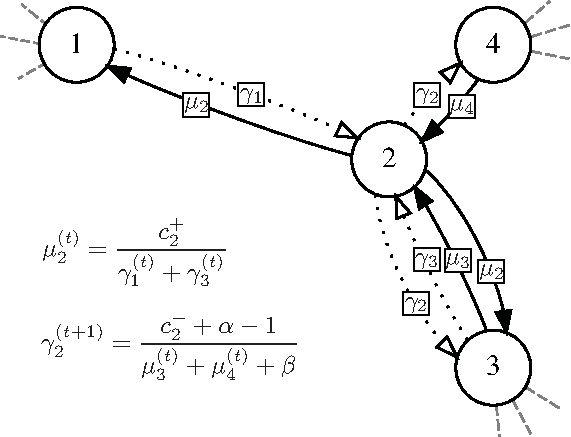
\includegraphics[scale=0.8]{cr-message-passing}
  \caption{One iteration of ChoiceRank from the perspective of node $2$.
  Messages flow in both directions along the edges of the graph $\mathcal{G}$, first in the reverse direction (in dotted) then in the forward direction (in solid).}
  \label{cr:fig:msgpassing}
\end{figure}

%%%%%%%%%%%%%%%%%%%%%%%%%%%%%%%%%%%%%%%%%%%%%%%%%%%%%%%%%%%%%%%%%%%%%%%%%
\subsection{EM Viewpoint}

The MM algorithm can also be interpreted from an expectation-maximization (EM) viewpoint, following the ideas of \citet{caron2012efficient}.
We introduce $N$ independent random variables $\mathcal{Z} = \{ z_i : i = 1, \ldots, N \}$, where
\begin{align*}
z_i \sim \text{Gamma} \bigg( c^+_i, \sum_{j \in \mathcal{N}^+_i} w_{ij} \gamma_j \bigg).
\end{align*}
With the addition of these latent random variables, the complete log-likelihood becomes
\begin{align*}
\ell(\bm{\gamma} ; \mathcal{D}, \mathcal{Z})
    &= \ell(\bm{\gamma}; \mathcal{D}) + \sum_{i = 1}^N \log p(z_i \mid \mathcal{D}, \bm{\gamma}) \\
    &= \sum_{i = 1}^N \bigg[ c^-_i \log \gamma_i - c^+_i \log \sum_{k \in \mathcal{N}^+_i} w_{ik} \gamma_k \bigg] \\
    &\qquad +\sum_{i = 1}^N \bigg[  c^+_i \log \sum_{k \in \mathcal{N}^+_i} w_{ik} \gamma_k - z_i \sum_{k \in \mathcal{N}^+_i} w_{ik} \gamma_k \bigg] + \kappa \\
    &= \sum_{i = 1}^N \bigg[ c^-_i \log \gamma_i - z_i \sum_{k \in \mathcal{N}^+_i} w_{ik} \gamma_k \bigg] + \kappa.
\end{align*}
Using a $\text{Gamma}(\alpha, \beta)$ prior for each parameter, the expected value of the log-posterior with respect to the conditional $\mathcal{Z} \mid \mathcal{D}$ under the estimate $\bm{\gamma}^{(t)}$ is
\begin{align*}
Q(\bm{\gamma}, \bm{\gamma}^{(t)})
    &= \mathbf{E}_{\mathcal{Z} \mid \mathcal{D}, \bm{\gamma}^{(t)}} \left[ \ell(\bm{\gamma} ; \mathcal{D}, \mathcal{Z}) \right]
       + \log p(\bm{\gamma}) \\
    &=\sum_{i = 1}^N \bigg[ c^-_i \log \gamma_i - c^+_i \frac{\sum_{k \in \mathcal{N}^+_i} w_{ik} \gamma_k}{\sum_{k \in \mathcal{N}^+_i} w_{ik} \gamma^{(t)}_k} \bigg]
      + \sum_{i = 1}^N \bigg[ (\alpha -1) \log \gamma_i - \beta \gamma_i \bigg] + \kappa.
\end{align*}
The EM algorithm starts with an initial $\bm{\gamma}^{(0)}$ and iteratively refines the estimate by solving the optimization problem $\bm{\gamma}^{(t+1)} = \Argmax_{\bm{\gamma}} Q(\bm{\gamma}, \bm{\gamma}^{(t)})$.
It is not difficult to see that for a given $\bm{\gamma}^{(t)}$, maximizing $Q(\bm{\gamma}, \bm{\gamma}^{(t)})$ is equivalent to maximizing the minorizing function $f^{(t)}(\bm{\gamma})$ defined in~\eqref{cr:eq:minorizing}.
Hence, the MM and the EM viewpoint lead to the exact same sequence of iterates.

The EM formulation leads to a Gibbs sampler in a relatively straightforward way \citep{caron2012efficient}.
We leave a systematic treatment of Bayesian inference in the network choice model for future work.
